\section{Quantum dynamics}
\label{sec:quantum}

\subsection{Floquet states and quasienergies}
\label{sec:floquet}

Because the Hamiltonian is periodic in time, the evolution over $n$ periods is just $\hat U^n$. The Floquet
operator is unitary, so its eigenvalues lie on the unit circle:
\begin{equation}
  \hat U|\phi_k\rangle = \ee^{-i\omega_k}|\phi_k\rangle, \qquad \omega_k \in [0, 2\pi).
\end{equation}
The phases $\omega_k$ are called quasienergies, and the $|\phi_k\rangle$ Floquet states. They play the role
that energy eigenstates play for a time-independent Hamiltonian. Expanding the initial state as
$|\psi_0\rangle = \sum_k c_k|\phi_k\rangle$ gives
\begin{equation}
  |\psi_n\rangle = \sum_k c_k\,\ee^{-in\omega_k}|\phi_k\rangle,
  \qquad
  \avg{p^2}_n = \sum_{k,k'} c_k^* c_{k'}\,\ee^{in(\omega_k - \omega_{k'})}\,\langle\phi_k|\hat p^2|\phi_{k'}\rangle.
  \label{eq:floquet_expansion}
\end{equation}
Whether the energy can grow without bound depends on the Floquet states. Suppose they are localized in
momentum, $|\phi_k(m)| \sim \ee^{-|m - m_k|/l}$ around some center $m_k$. Then a state started at $m = 0$
overlaps appreciably only with the Floquet states centered within a few $l$ of the origin, so in effect the
sum in \cref{eq:floquet_expansion} has finitely many terms. The energy is then a quasi-periodic function of
$n$: it fluctuates, but it is bounded. Its time average keeps only the diagonal terms (if no two quasienergies
coincide),
\begin{equation}
  \overline{\avg{p^2}} = \sum_k |c_k|^2\,\langle\phi_k|\hat p^2|\phi_k\rangle,
  \qquad
  \overline{P}(m) = \sum_k |c_k|^2\,|\phi_k(m)|^2,
  \label{eq:time_average}
\end{equation}
where $\overline{P}(m)$ is the time-averaged momentum distribution. If instead the spectrum has a
continuous part, with Floquet states extended in momentum, the energy can grow forever. So the question
``does the quantum energy keep growing?'' becomes ``are the Floquet states localized?'' The two exactly
solvable cases below show both possibilities, and the Anderson mapping in \cref{sec:anderson} explains why
localization is the generic answer.

\subsection{Quantum resonance and antiresonance}
\label{sec:resonance}

For special values of $\hbar$ the free phase $\ee^{-i\hbar m^2/2}$ simplifies. At $\hbar = 4\pi$ it equals
$\ee^{-2\pi i m^2} = 1$ for every $m$: the free evolution does nothing, and all kicks add up coherently.
After $n$ kicks the wave function is $\ee^{-inK\cos\theta/\hbar}$, so by the Jacobi-Anger expansion
\begin{equation}
  |\psi_m|^2 = J_m^2(nK/\hbar), \qquad
  \avg{p^2}_n = \hbar^2\sum_m m^2 J_m^2(nK/\hbar) = \frac{K^2 n^2}{2}.
  \label{eq:resonance}
\end{equation}
The energy grows quadratically: the motion is ballistic, faster than any diffusion. This \emph{quantum
resonance} was found by Casati et al.\ \cite{Casati1979}, who also saw quadratic growth at several other
rational values of $\hbar/4\pi$. For a rational $\hbar/4\pi = r/q$ the free phases repeat with period $q$ in
$m$, the Floquet states become extended Bloch waves, and the energy grows without bound
\cite{Izrailev1980,Izrailev1990}.

At $\hbar = 2\pi$ the free phase is $\ee^{-i\pi m^2} = (-1)^m$, which shifts the wave function by $\pi$ in
angle. The next kick then sees $\cos(\theta + \pi) = -\cos\theta$ and undoes the previous one, so
$\hat U^2 = 1$: every state returns exactly after two kicks, for any $K$. Casati et al.\ called this case
``anti-resonant'' \cite{Casati1979}. The energy alternates between $K^2/2$ and 0.

\begin{figure}[!tbp]
  \centering
  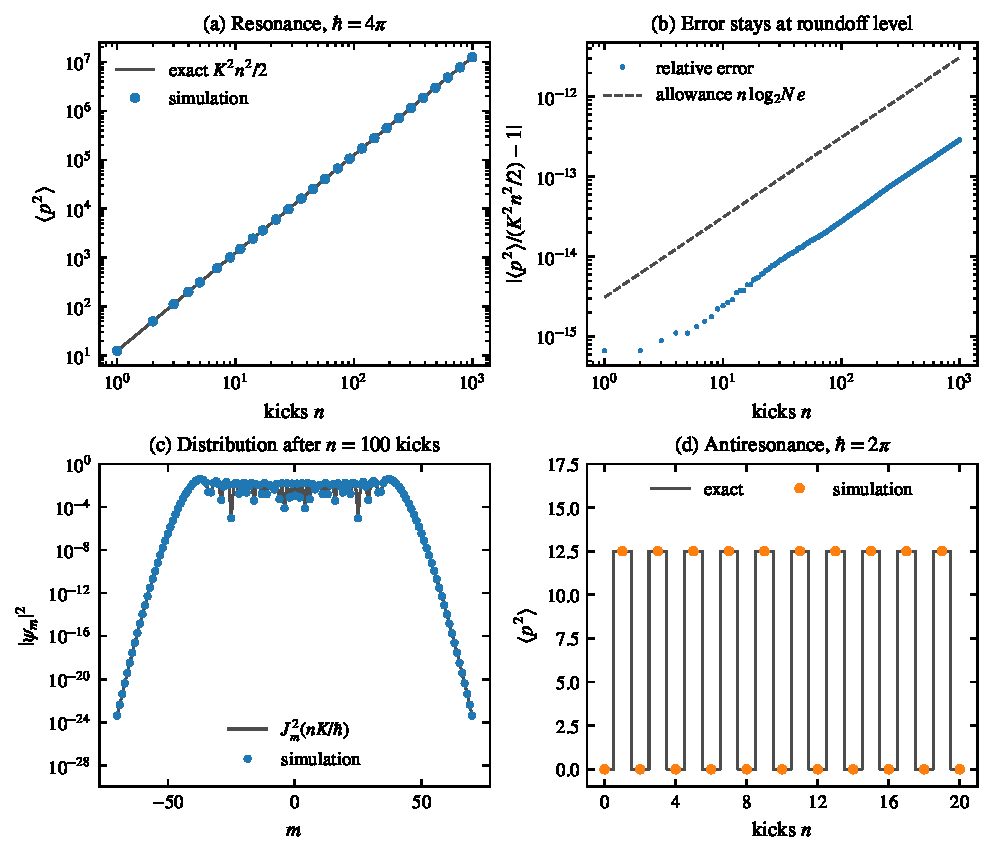
\includegraphics[width=0.85\linewidth]{05_resonance_test.pdf}
  \caption{Quantum resonance and antiresonance at $K = 5$ (experiment 05, validation check 2).
  (a) At $\hbar = 4\pi$ the energy grows as $K^2n^2/2$. (b) The relative error stays below the roundoff
  allowance $n\log_2 N\,\varepsilon$ for $N = 2^{14}$. (c) After 100 kicks the momentum distribution is
  $J_m^2(nK/\hbar)$ over 28 decades. (d) At $\hbar = 2\pi$ the state returns to $m = 0$ after every second
  kick.}
  \label{fig:resonance}
\end{figure}

These exact results make an ideal test of the code (\cref{fig:resonance}). Over 1000 kicks at
$\hbar = 4\pi$ the simulated energy stays within a relative $2.9\times10^{-13}$ of $K^2n^2/2$, an error that
grows linearly with $n$ as roundoff should, and after 100 kicks the distribution matches $J_m^2(nK/\hbar)$
within $1.7\times10^{-15}$. At $\hbar = 2\pi$ the state returns to $m = 0$ within $2.8\times10^{-15}$.

The resonances also tell us what to avoid. In the localization runs, $\hbar/4\pi$ must be irrational and not
too close to a rational with a small denominator. All our standard values ($\hbar = 0.25$, 0.5 and 1) satisfy
this. \Cref{sec:scaling} shows what happens when it fails.

\subsection{Early times: quantum follows classical}
\label{sec:early}

After one kick both theories give exactly $\avg{p^2}_1 = K^2/2$. After two kicks they first differ
(\cref{app:two_kicks}):
\begin{align}
  \avg{p^2}_2^{\rm cl} &= K^2\bigl[1 + J_0(K) - J_2(K) - \tfrac12 J_2(2K)\bigr], \label{eq:two_kicks_cl}\\
  \avg{p^2}_2^{\rm qm} &= K^2\bigl[1 + \cos\tfrac{\hbar}{2}\,\bigl(J_0(K_q) - J_2(K_q)\bigr) - \tfrac12 J_2(K_2)\bigr],
  \qquad K_q = \tfrac{2K}{\hbar}\sin\tfrac{\hbar}{2},\quad K_2 = \tfrac{2K}{\hbar}\sin\hbar. \label{eq:two_kicks_qm}
\end{align}
As $\hbar \to 0$, $K_q \to K$ and $K_2 \to 2K$, and the quantum result goes over into the classical one.
The difference is of order $\hbar^2$: at $K = 5$ the quantum value is lower by 0.18\% at $\hbar = 0.1$ and by
1.0\% at $\hbar = 0.25$. (At $\hbar = 4\pi$ the formula gives $2K^2$, the resonance value, and at
$\hbar = 2\pi$ it gives 0, the antiresonance.) Both formulas are reproduced by the code to machine precision
(check 3).

At later times the agreement deteriorates quickly. Since $\avg{p^2}$ is even in $\hbar$, the quantum value
approaches the classical one as $c + a\hbar^2 + O(\hbar^4)$, but the coefficient $a$ grows rapidly with the
number of kicks: about $-0.2$ at $n = 2$, $-35$ at $n = 3$ and roughly $-550$ at $n = 4$ (relative to the
classical value, $K = 5$). At $\hbar = 0.05$ the three-kick gap is already 6\%. This is the Ehrenfest time at
work: chaotic stretching magnifies quantum effects by about $\ee^{\lambda}$ per kick, so detailed
correspondence lasts only for $t_E \sim \lambda^{-1}\ln(1/\hbar)$, a few kicks here; after that ``only rough
statistical properties like diffusion remain'' \cite{Izrailev1990}. The correspondence limit still holds at
fixed $n$: from $\hbar = 0.02$, 0.01 and 0.005 the gap at $n = 3$ shrinks with an observed order of 1.97 in
$\hbar$, and a Richardson extrapolation recovers the classical $\avg{p^2}_3 = 32.25286$ within
$1.2\times10^{-4}$ (check 3).

\subsection{Dynamical localization}
\label{sec:localization}

Diffusion survives the Ehrenfest time, but not forever. A simple estimate shows when it must stop. Suppose
the Floquet states are localized with a length of order $\xi$ momentum states. Then the initial state
overlaps with roughly $\xi$ of them, and their quasienergies, spread over $[0, 2\pi)$, have a mean spacing of
about $2\pi/\xi$. The evolution cannot resolve this spacing before a time of order $t^* \sim \xi$ kicks (the
analog of the Heisenberg time $\hbar/\Delta E$). Before $t^*$ the dynamics does not know the spectrum is
discrete, and the momentum diffuses as in the classical system, $\avg{m^2} \approx Dn/\hbar^2$; after $t^*$ it
stops. Consistency requires $\xi^2 \sim \avg{m^2}(t^*) \sim Dt^*/\hbar^2 \sim D\xi/\hbar^2$, so
\begin{equation}
  \xi \sim \frac{D}{\hbar^2}, \qquad t^* \sim \frac{D}{\hbar^2}, \qquad
  \avg{p^2}_\infty \sim \hbar^2\xi^2 \sim \frac{D^2}{\hbar^2}.
  \label{eq:estimates}
\end{equation}
The localization length is the classical diffusion rate measured in momentum states per kick. The smaller
$\hbar$, the longer the classical-like growth lasts and the higher the energy at which it saturates, but for
any $\hbar > 0$ the growth eventually stops. The classical limit $\hbar\to0$ and the long-time limit
$n\to\infty$ do not commute.

\begin{figure}[!tbp]
  \centering
  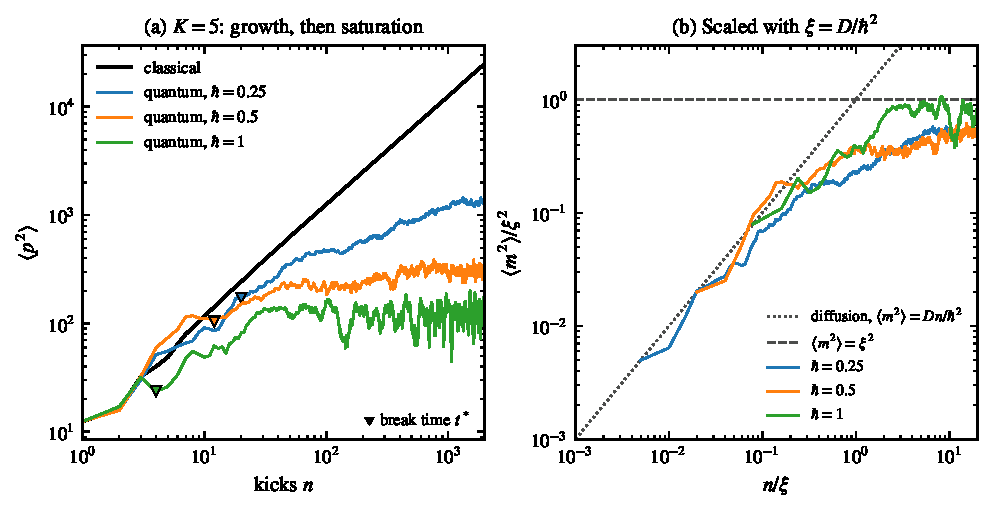
\includegraphics[width=\linewidth]{03_quantum_vs_classical.pdf}
  \caption{The main result (experiment 03, $K = 5$). (a) The classical energy (black, 40000 orbits) grows
  linearly forever. The quantum energy (colors, starting in $m = 0$) follows it at first and then saturates;
  triangles mark the break time $t^*$, after which the quantum energy stays more than 25\% below the classical
  one. (b) The same curves in units of $\xi = D/\hbar^2$: $\avg{m^2}/\xi^2$ against $n/\xi$. The dotted line is
  the diffusive growth $\avg{m^2} = Dn/\hbar^2$, the dashed line $\avg{m^2} = \xi^2$.}
  \label{fig:quantum_vs_classical}
\end{figure}

\Cref{fig:quantum_vs_classical} shows exactly this behavior (experiment 03). The classical ensemble diffuses
with $D = 12.51 \pm 0.10$, that is, $D/(K^2/2) = 1.001$. The quantum curves for $\hbar = 0.25$, 0.5 and 1
follow it and then bend over and saturate. We define the break time as Izrailev does \cite{Izrailev1990}: the
first kick from which the quantum energy stays more than 25\% below the classical one. This gives
$t^* = 20$, 12 and 4 kicks, or 0.10, 0.24 and 0.32 times $\xi = D/\hbar^2$; the estimate $t^* \sim \xi$ is only
an order of magnitude, and with this criterion the break comes earlier. Averaged over kicks 1000 to 2000, the
saturated energies are 1305, 300 and 119, which is 0.52, 0.48 and 0.76 times $D^2/\hbar^2$. For
$\hbar = 0.25$, Izrailev's Fig.~1 shows the same case over 2000 kicks; read off the figure, his energy levels
off near $\avg{p^2} \approx 1400$, consistent with ours.

The saturated energy is not constant. In a run of 40000 kicks at $\hbar = 0.25$, the averages over blocks of
2500 kicks ranged from 1100 to 1960 around a mean of about 1500 (17\% rms), with no upward trend. Such slow
swings are what \cref{eq:floquet_expansion} predicts: the energy is a sum of terms oscillating at the
differences of nearby quasienergies, some of which are very small.

Panel (b) of \cref{fig:quantum_vs_classical} rescales the curves with $\xi = D/\hbar^2$. Diffusion is then
the same line for all three values of $\hbar$, and all three curves leave it near $n/\xi \approx 0.1$ and
level off between 0.5 and 1 times $\xi^2$. The collapse is not perfect, but it confirms that $\xi$ sets both
the break time and the saturation level.

\subsection{The localized momentum distribution}
\label{sec:distribution}

The time-averaged momentum distribution \cref{eq:time_average} is the clearest signature of localization.
If the Floquet states were simple exponentials with a fixed length, $\overline{P}(m)$ would be a sum of
exponentials. Shepelyansky \cite{Shepelyansky1986} found that the Floquet states decay like
$|\phi(m)|^2 \sim \ee^{-2|m|/l}$ with $l \approx D/(2\hbar^2)$, and that the time-averaged distribution of a
state started at $m = 0$ decays about twice as slowly, because the Floquet states fluctuate strongly; from
Chirikov and Shepelyansky's data its length is $l_s = (1.04 \pm 0.20)\,D/\hbar^2$ (mean and rms spread).
Izrailev \cite{Izrailev1990} gives its shape,
\begin{equation}
  \overline{P}(m) = \frac{1}{2\xi}\Bigl(1 + \frac{2|m|}{\xi}\Bigr)\ee^{-2|m|/\xi},
  \qquad \avg{m^2} = \xi^2,
  \label{eq:izrailev_shape}
\end{equation}
with $\xi = l_s \approx D/\hbar^2$. This defines our localization length: $|\psi_m|^2 \sim \ee^{-2|m|/\xi}$
in the tails. (Moore et al.\ \cite{Moore1995} define the localization length as the $1/e$ point of the
probability, which is half of ours.) The prefactor matters for fitting: fitting a pure exponential to
\cref{eq:izrailev_shape} overestimates $\xi$ by 31\% over $\xi/2 \le |m| \le 3\xi$ and still by 7\% over
$4\xi \le |m| \le 10\xi$. So we fit the full shape, in $\ln\overline{P}$, from $|m| = 5$ (past the central
peak) out to where $\overline{P}$ falls to $10^{-14}$ of its maximum.

\begin{figure}[!tbp]
  \centering
  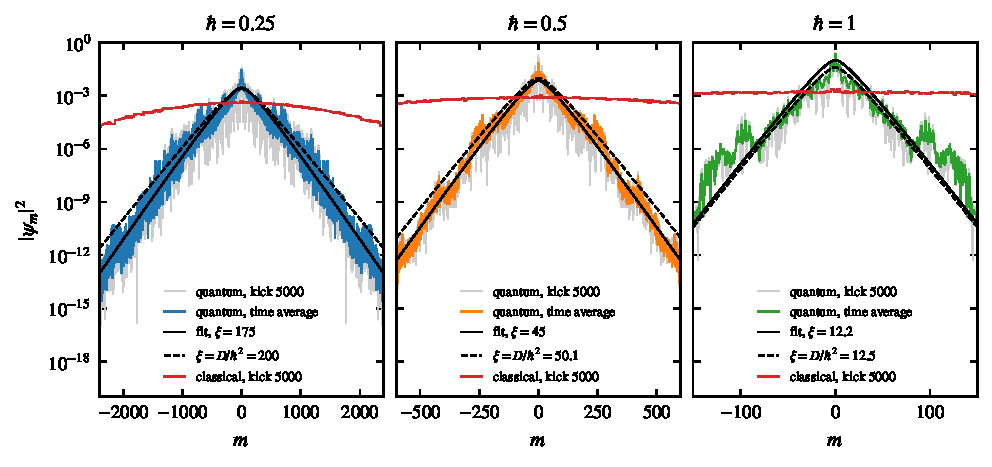
\includegraphics[width=\linewidth]{04_momentum_distribution.pdf}
  \caption{The localized momentum distribution at $K = 5$ (experiment 04). Colors: the quantum distribution
  averaged over kicks 2500 to 5000; gray: the distribution at kick 5000; black solid: the fit of
  \cref{eq:izrailev_shape}; black dashed: the same shape with $\xi = D/\hbar^2$; red: the classical
  distribution at kick 5000 (bins with fewer than 10 of the 40000 orbits are not drawn). Note the 20 decades
  on the vertical axis.}
  \label{fig:distribution}
\end{figure}

\Cref{fig:distribution} shows the result (experiment 04). On a logarithmic scale the quantum distributions
are straight-sided tents: exponential localization, over 13 decades at $\hbar = 0.25$. The classical
distribution at the same time is a broad Gaussian, nearly flat on this scale, with width
$\sqrt{Dn}/\hbar = 1000$ states at $\hbar = 0.25$ and still growing like $\sqrt n$. The fitted localization
lengths are 175, 45.0 and 12.2 states, or 0.87, 0.90 and 0.98 times $D/\hbar^2$, inside the spread of
Shepelyansky's data. Three caveats come with these numbers:
\begin{itemize}
  \item The far tails fill in slowly, so the fit depends on the averaging window. Averaging over kicks 1000 to
  2000 instead gives 0.80, 0.84 and 0.97. A 40000-kick run at $\hbar = 0.25$ levels off at 0.90 to 0.92 for
  windows from 5000 kicks on: the tail at $|m| \approx 3000$ (about $15\xi$) rises from $10^{-17.7}$ in the
  early window to about $10^{-14.6}$ and then stays there.
  \item At $\hbar = 1$ only about a dozen states are involved and the distribution is bumpy: fitting only the
  inner half of the range gives 17 to 18.5 instead of 12.2.
  \item The distributions have a narrow central peak that \cref{eq:izrailev_shape} lacks. The states
  $|m| < 5$ hold 9\% of the probability at $\hbar = 0.25$ and 19\% at $\hbar = 0.5$, against 3\% and 6\% under
  the fitted shape. This is why $\sqrt{\avg{m^2}}$ (154 and 34) comes out below the fitted $\xi$ (175 and 45).
  We have not identified its cause.
\end{itemize}
The distribution at a single kick (gray) fluctuates strongly around the time average. These fluctuations are
the beats between nearby quasienergies in \cref{eq:floquet_expansion}, and they can be large: at
$\hbar = 0.25$ the states near $|m| \approx 680$ hold up to 1.3\% of the probability around kick 1500, more
than twice their time average of 0.6\%, before it drains away again. An animation of the distribution, quantum against classical, is in
\texttt{figures/04\_momentum\_distribution.gif}: the classical Gaussian keeps widening while the quantum
tent stops spreading after a few hundred kicks.

\subsection{How the localization length scales with \texorpdfstring{$\hbar$}{hbar} and \texorpdfstring{$K$}{K}}
\label{sec:scaling}

Experiment 07 tests $\xi \approx D/\hbar^2$ over a wider range (\cref{fig:scaling}). Each run starts in
$m = 0$, lasts at least 5000 kicks and at least $50\,D/\hbar^2$ kicks, and fits \cref{eq:izrailev_shape} to
the time average over its second half. The grid is enlarged until the edge probability stays below
$10^{-10}$ and the fit range lies well inside it. The classical $D$ is measured at each $K$ with the matched
ensemble, and $K$ is kept away from the accelerator windows and from $K = 9.25$ (\cref{sec:diffusion}).

\begin{figure}[!tbp]
  \centering
  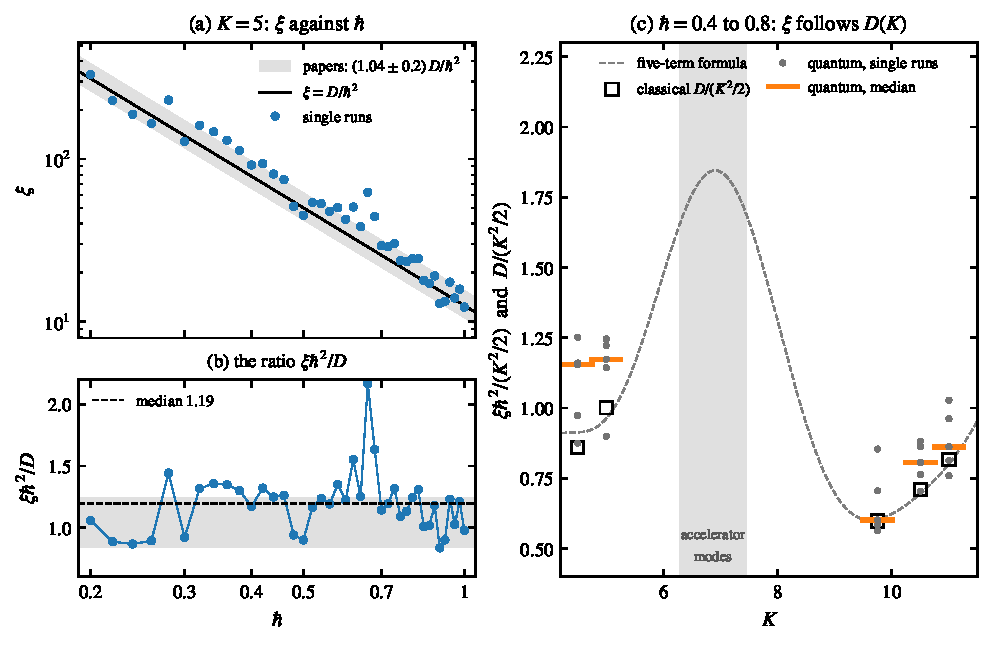
\includegraphics[width=\linewidth]{07_bonus_xi_scaling.pdf}
  \caption{Scaling of the localization length (experiment 07). (a) $\xi$ against $\hbar$ at $K = 5$ for 41
  single runs, with $\xi = D/\hbar^2$ (line) and Shepelyansky's $(1.04\pm0.20)\,D/\hbar^2$ (band). (b) The
  ratio $\xi\hbar^2/D$ for the same runs. (c) $\xi\hbar^2/(K^2/2)$ for five values of $\hbar$ between 0.4 and
  0.8 (dots) and their median (bars), against the measured classical $D/(K^2/2)$ (squares) and the five-term
  formula \cref{eq:five_term} (dashed).}
  \label{fig:scaling}
\end{figure}

Panel (a) shows 41 runs at $K = 5$ with $\hbar$ from 0.20 to 1.00. While $\xi$ falls by a factor of about
27, from 330 to 12, it follows $D/\hbar^2$ closely. Panel (b) shows the ratio $\xi\hbar^2/D$: its median is
1.19 and its rms spread 0.25, compared with $1.04 \pm 0.20$ from Shepelyansky's data. The scatter is not
random from point to point, though. The ratio wanders in broad bands, about 0.89 for $\hbar < 0.3$, about 1.25
from 0.3 to 0.75 and about 1.09 above, and values of $\hbar$ only 0.01 apart give strongly correlated
results (correlation coefficient 0.57 between neighbors in a finer scan). We do not know the cause of these
bands. The known quantum correction to the diffusion rate, replacing $K$ by $K_q$ in the Bessel functions
\cite{Izrailev1990}, changes $D$ by only about 2\% at $\hbar = 0.35$, far too little.

Panel (c) varies the kick strength at fixed $\hbar$. The naive estimate $D = K^2/2$ would make
$\xi\hbar^2/(K^2/2)$ constant. Instead it follows the measured classical $D/(K^2/2)$: about 1.15 at
$K = 4.5$ and 5, then down to 0.60 at $K = 9.75$, exactly where the classical diffusion has its Bessel dip
(0.60), and back up to 0.81 and 0.86 at $K = 10.5$ and 11. The quantum localization length inherits the
oscillations of the classical diffusion rate.

Finally, a warning about resonances. In an earlier version of this experiment, one run at $\hbar = 0.714$
gave $\xi\hbar^2/D = 4.8$ and pushed probability to the edge of a 2048-state grid. The reason is arithmetic:
$0.714/4\pi$ differs from $5/88$ by only $1.4\times10^{-7}$, so the free phases repeat with period 88 out to
$|m| \sim 1000$, and the state spreads as if at a resonance. The final version of the experiment would report such a run as
not localized instead of fitting it; none of the runs in \cref{fig:scaling} needed that.

\subsection{The Anderson localization analogy}
\label{sec:anderson}

Why are the Floquet states localized? Fishman, Grempel and Prange \cite{Fishman1982} answered this by
turning the Floquet eigenvalue problem into a tight-binding model. Write the kick as
\begin{equation}
  \ee^{-ik\cos\theta} = \frac{1 + iW(\theta)}{1 - iW(\theta)}, \qquad W(\theta) = -\tan\Bigl(\frac{k\cos\theta}{2}\Bigr),
  \qquad k = \frac{K}{\hbar},
\end{equation}
and look for a Floquet state $\hat U|u\rangle = \ee^{-i\omega}|u\rangle$ in the form $u = (1 - iW)v$. The free
phases are diagonal in $m$, and a few lines of algebra turn the eigenvalue equation into
\begin{equation}
  T_m v_m + \sum_{r\ne0} W_r\,v_{m+r} = -W_0\,v_m,
  \qquad T_m = \tan\Bigl(\frac{\omega - \hbar m^2/2}{2}\Bigr),
  \label{eq:anderson}
\end{equation}
where $W_r$ are the Fourier coefficients of $W(\theta)$. This is the equation for a particle hopping on a
one-dimensional lattice, whose sites are the momentum states $m$. The hopping amplitudes $W_r$ come from the
kick, and $T_m$ plays the role of an on-site energy.

When $\hbar/4\pi$ is irrational, the phases $\hbar m^2/2 \bmod 2\pi$ are spread uniformly and in an
irregular order, so $T_m$, the tangent of a uniformly distributed angle, behaves like a random number with a
Cauchy (Lorentzian) distribution. \Cref{eq:anderson} is then the Lloyd model, a version of the Anderson model
of a particle in a random potential, in which all eigenstates in one dimension are exponentially localized.
The localized Floquet states in momentum are the analog of localized electron states in a disordered wire,
with the time-periodic kicking playing the role of the disorder. When $\hbar/4\pi$ is rational, $T_m$ is
periodic in $m$, the eigenstates are extended Bloch waves, and the energy grows: the quantum resonance of
\cref{sec:resonance}. The ``disorder'' here is deterministic, though, which is why the arithmetic of
$\hbar/4\pi$ matters, as the near-resonant run of \cref{sec:scaling} showed.

The analogy explains why the Floquet states are localized, but not how long they are. For that we need the
diffusion argument of \cref{sec:localization} and numerical results such as Shepelyansky's
$l \approx D/(2\hbar^2)$ for the Floquet states \cite{Shepelyansky1986} and the measurements of
\cref{sec:distribution,sec:scaling}.
